\documentclass{article}
\usepackage{amsmath,amssymb,graphics}
\usepackage{color}
% \VignetteIndexEntry{Population Stochastic Modelling: Model definition, description and examples}
% \VignetteDepends{PSM}

\newcommand{\bs}{\boldsymbol}

\usepackage{boxedminipage}

\usepackage{/appl/R/R-2.6.2/lib64/R/share/texmf/Sweave}
%%%
% look and feel of the R code
%%%
\DefineVerbatimEnvironment{Sinput}{Verbatim}{fontsize=\small,fontshape=sl}
\DefineVerbatimEnvironment{Soutput}{Verbatim}{fontsize=\small}
\DefineVerbatimEnvironment{Scode}{Verbatim}{fontsize=\small,fontshape=sl}
%%%
% put R code and R-code output in a boxed minipage:
%%%
\definecolor{light}{gray}{.75} 
\renewenvironment{Schunk}
{\begin{center} \begin{boxedminipage}{0.95\textwidth} }
{\end{boxedminipage}\end{center}}


\usepackage{/appl/R/R-2.6.2/lib64/R/share/texmf/Sweave}
\begin{document}


\title{Population Stochastic Modelling (PSM): \\
Comparison with CTSM} 

\date{\today}

\author{Stig Mortensen and S\o ren Klim}
\maketitle

\begin{center}
\begin{tabular}{lp{6cm}}
Package:& PSM, version 0.8-1\\
URL:    & http://www.imm.dtu.dk/psm 
\end{tabular}
\end{center}

\vspace{.2cm}

%\setcounter{tocdepth}{1}
\tableofcontents

\vspace{.2cm}


\section{Purpose}

The first stage model of PSM is based on the stochastic state space
model defined in CTSM. For 'single-subject' data in a model without
random effects the two programs should therefore give equal state
estimates and likelihood function.

This document compares the estimation results of PSM and
CTSM\cite{kristensen03} for a fed-batch bioreactor example. The model
is specified in the CTSM User's Guide\cite{kristensen03b} on page 55.
The comparison is based on simulated data created in CTSM for a single
bioreactor.

\newpage

\section{Setting up the example}

The non-linear model contains three states $X$, $S$ and $V$ which are
the biomass concentration, the substrate concentration and the volume.
It has one input $F$ which is the feed flow rate. There are three
output/response variable $y1$, $y2$ and $y3$ which directly observes
the tree states.

\subsection{Loading data}

Initially the data is loaded from the original file \verb|sde0_1.csv|
created by CTSM. The data file is contained in the examples folder in
CTSM.

\begin{Schunk}
\begin{Sinput}
> library(PSM)
> tmpData <- read.table("sde0_1.csv", sep = ";", 
+     col.names = c("Time", "F", "y1", "y2", "y3"))
> Time = tmpData$Time
> Y = t(tmpData[, c("y1", "y2", "y3")])
> U = t(as.matrix(tmpData[, c("F")]))
> Data <- list(Time = Time, Y = Y, U = U)
\end{Sinput}
\end{Schunk}


\subsection{Model specification}

The model object is specified in R as follows.
\newpage

\begin{Schunk}
\begin{Sinput}
> MyModel <- list()
> MyModel$X0 = function(Time, phi, U) {
+     matrix(c(phi$x0, phi$s0, phi$v0), ncol = 1)
+ }
> MyModel$h = function(eta, theta, covar) {
+     phi = theta
+ }
> MyModel$Functions$f = function(x, u, time, phi) {
+     X <- x[1]
+     S <- x[2]
+     V <- x[3]
+     F <- u[1]
+     mu <- phi$mumax * S/(phi$k2 * S^2 + S + phi$k1)
+     matrix(c(mu * X - F * X/V, -mu * X/phi$Y + 
+         F * (phi$sf - S)/V, F), ncol = 1)
+ }
> MyModel$Functions$df = function(x, u, time, phi) {
+     X <- x[1]
+     S <- x[2]
+     V <- x[3]
+     F <- u[1]
+     kssk = (phi$k2 * S^2 + S + phi$k1)
+     matrix(c(phi$mumax * S/kssk - F/V, phi$mumax/kssk * 
+         X - phi$mumax * S/(kssk)^2 * X * (2 * 
+         phi$k2 * S + 1), F * X/V^2, -phi$mumax * 
+         S/(kssk)/phi$Y, -phi$mumax/(kssk) * X/phi$Y + 
+         phi$mumax * S/(kssk)^2 * X/phi$Y * (2 * 
+             phi$k2 * S + 1) - F/V, -F * (phi$sf - 
+         S)/V^2, 0, 0, 0), nrow = 3, ncol = 3, 
+         byrow = TRUE)
+ }
> MyModel$Functions$g = function(x, u, time, phi) {
+     x
+ }
> MyModel$Functions$dg = function(x, u, time, phi) {
+     diag(3)
+ }
> MyModel$S = function(u, time, phi) {
+     diag(c(phi$s11, phi$s22, phi$s33))
+ }
> MyModel$SIG = function(u, time, phi) {
+     diag(c(phi$sig11, phi$sig22, phi$sig33))
+ }
\end{Sinput}
\end{Schunk}

\section{Results of comparison}

\subsection{Likelihood function value}

The objective functions of PSM and CTSM are both the negative
log-likelihood function. The two are compared based ML-estimated
parameters found by CTSM. These parameter estimates are copied from
CTSM and specified below. At the same time the model is prepared to
estimate 5 of these parameters (\verb|mumax|, \verb|k1|, \verb|s11|,
\verb|s22| and \verb|s33|) later in this comparison.

\begin{Schunk}
\begin{Sinput}
> ctsmTHETA <- c(mumax = 1.0022, k1 = 0.031629, 
+     s11 = 0.0075248, s22 = 0.0010636, s33 = 0.011388)
> MyModel$ModelPar = function(THETA) {
+     list(theta = list(mumax = THETA["mumax"], 
+         k1 = THETA["k1"], k2 = 0.5, Y = 0.5, sf = 10, 
+         sig11 = 9.6704e-28, sig22 = 1.7471e-06, 
+         sig33 = 1.0903e-08, s11 = THETA["s11"], 
+         s22 = THETA["s22"], s33 = THETA["s33"], 
+         x0 = 1.0095, s0 = 0.23835, v0 = 1.004))
+ }
> theta <- MyModel$ModelPar(ctsmTHETA)$theta
\end{Sinput}
\end{Schunk}

The value of the CTSM negative log-likelihood function based on the
parameters above are 

\begin{equation}
  \text{CTSM:} \quad -\log L (\theta)= -388.4857 ~~.
  \label{ctsmL}
\end{equation}

The negative log-likelihood function in PSM can be evaluated by
directly calling the Extended Kalman Filter using the same
parameter values

\begin{Schunk}
\begin{Sinput}
> (negLogL <- ExtKalmanFilter(theta, MyModel, Data))
\end{Sinput}
\begin{Soutput}
[1] -388.4689
\end{Soutput}
\end{Schunk}

\noindent and the result can be seen to be very similar to the value found by
CTSM as shown in Equation \eqref{ctsmL}.

\subsection{Uncertainty for parameter estimates}


In CTSM parameter uncertainty is given by standard deviation (SD)
estimates for each parameter. In PSM parameter uncertainty is given by
either SD or a 95\% Wald confidence interval based on the Hessian of
the log-likelihood function.

To find the confidence intervals in PSM a parameter search is started
with an initial guess 10\% away from the CTSM ML-estimates. 

\begin{Schunk}
\begin{Sinput}
> MyPar <- list(LB = 0.5 * ctsmTHETA, Init = ctsmTHETA * 
+     1.1, UB = 1.5 * ctsmTHETA)
\end{Sinput}
\end{Schunk}

The parameter estimation is performed using the function PSM.estimate
which returns the negative log-likelihood value, ML-estimates and the
Wald confidence intervals. The result from PSM.estimate is shown below.

\begin{Schunk}
\begin{Sinput}
> (fit <- PSM.estimate(MyModel, list(Data), MyPar, 
+     CI = TRUE)[1:5])
\end{Sinput}
\begin{Soutput}
$NegLogL
[1] -388.5

$THETA
   mumax       k1      s11      s22      s33 
1.002231 0.031629 0.007530 0.001064 0.011429 

$CI
            mumax      k1      s11       s22      s33
Lower CI95 0.9937 0.02876 0.005452 0.0007663 0.008277
MLE        1.0022 0.03163 0.007530 0.0010640 0.011429
Upper CI95 1.0108 0.03450 0.009608 0.0013617 0.014581

$SD
        mumax       k1      s11       s22      s33
[1,] 0.004377 0.001465 0.001060 0.0001519 0.001608

$COR
           mumax         k1        s11       s22        s33
mumax  1.000e+00  9.975e-01  3.391e-02 1.680e-01 -1.844e-10
k1     9.975e-01  1.000e+00  3.388e-02 1.675e-01 -1.874e-10
s11    3.391e-02  3.388e-02  1.000e+00 5.697e-03 -8.954e-11
s22    1.680e-01  1.675e-01  5.697e-03 1.000e-00  2.589e-10
s33   -1.844e-10 -1.874e-10 -8.954e-11 2.589e-10  1.000e-00
\end{Soutput}
\end{Schunk}


The corresponding ML estimates and SD estimates in CTSM are copied
from the CTSM output and shown below. The estimates in PSM and CTSM
can be seen to be almost equal.

\begin{Schunk}
\begin{Sinput}
> ctsmEstimates
\end{Sinput}
\begin{Soutput}
       mumax       k1       s11       s22      s33
MLE 1.002200 0.031629 0.0075248 0.0010636 0.011388
SD  0.003342 0.001598 0.0009762 0.0001376 0.001496
\end{Soutput}
\end{Schunk}

To visually compare the error estimates in PSM and CTSM a Wald confidence interval
is generated from CTSM as MLE$\pm 1.96 \cdot$SD. This result of the
comparison is shown if Figure \ref{fig:fig1}.


\begin{figure}[hptb]
\begin{center}
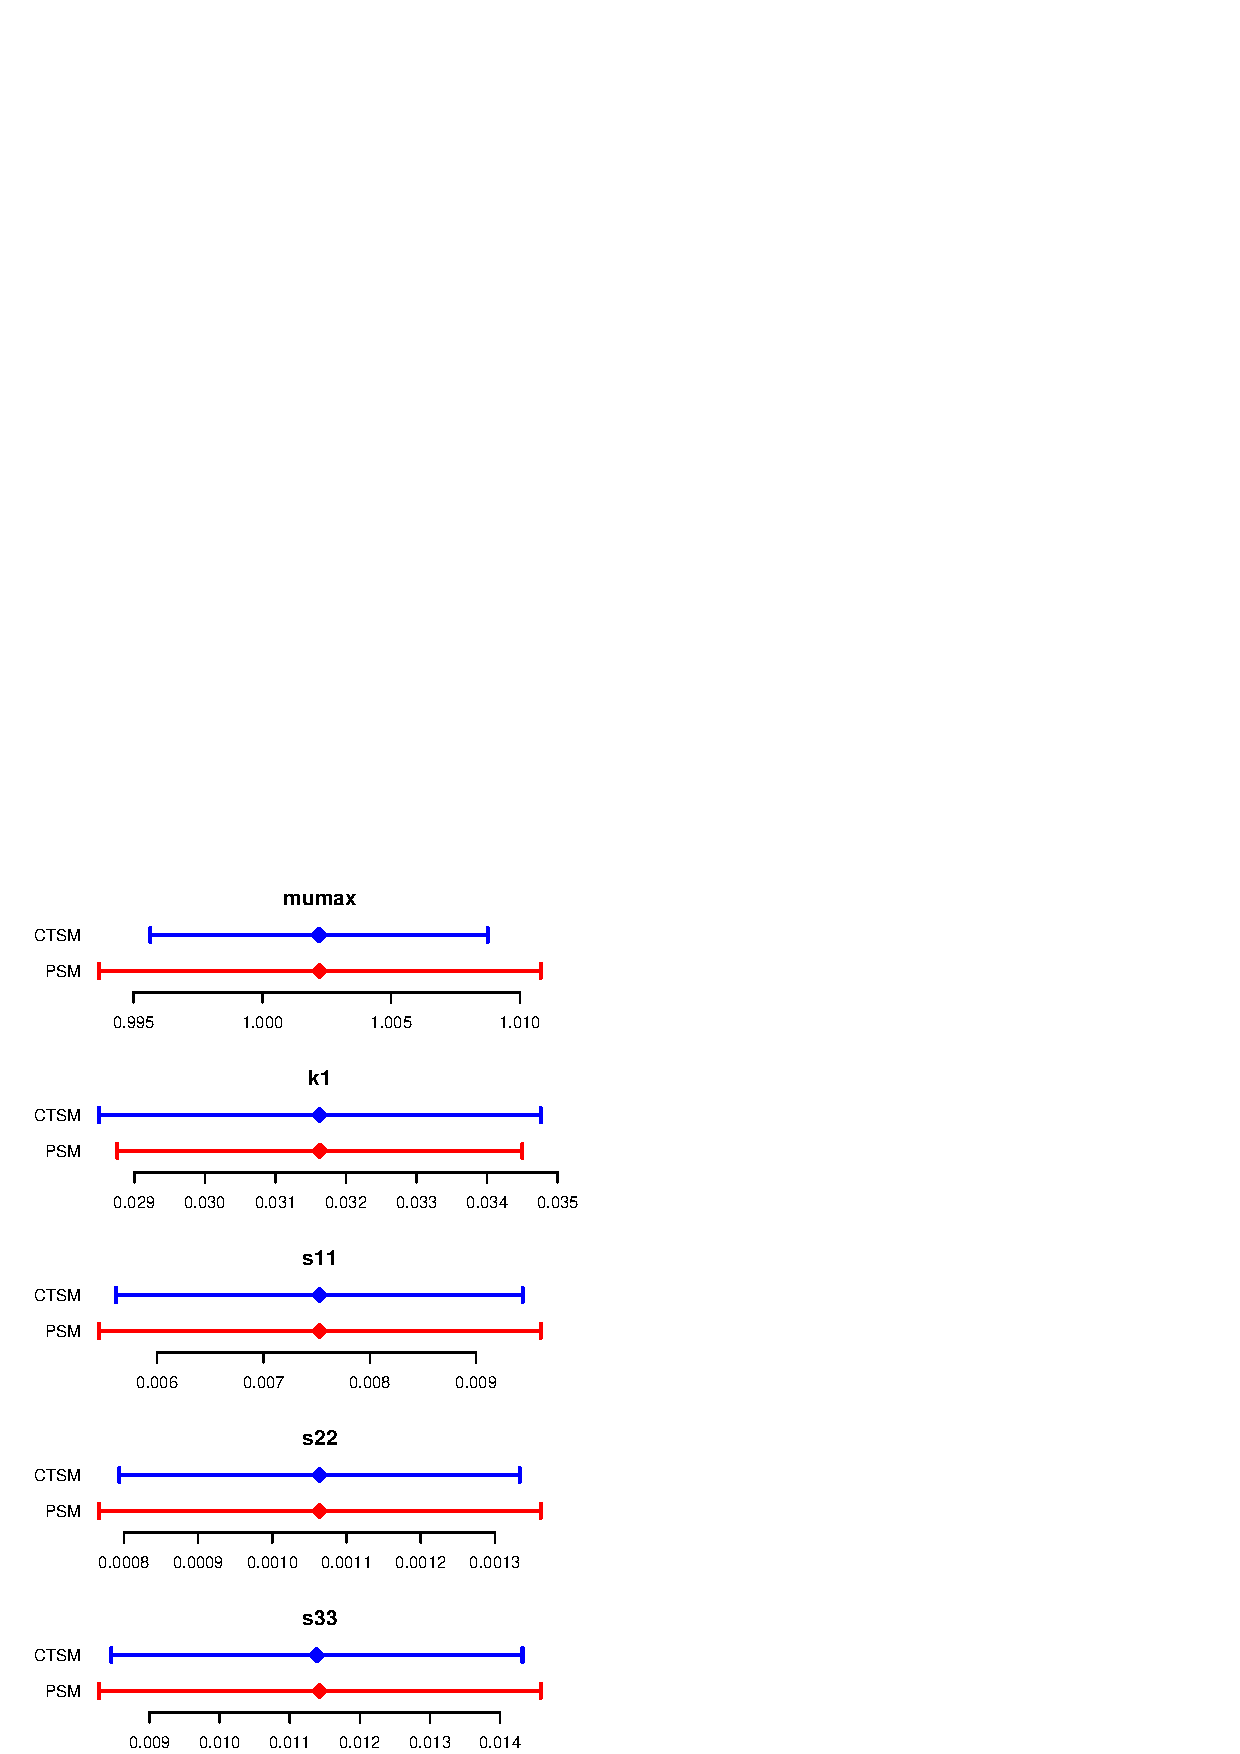
\includegraphics{PSMvsCTSM-figure1}
\end{center}
\caption{Visual comparison of error estimates for ML-estimated parameters in
  PSM and CTSM.}
\label{fig:fig1}
\end{figure}

\newpage

\subsection{State estimates}

The state estimates in PSM and CTSM should also be equal. This is
expected to be the case for the state and state covariance one-step
predictions since the likelihood function is evaluated
based on these.

The smoothed state estimate is the optimal state estimate where all
data is used at each time point. To compare these a smoothed state
estimate is generated in CTSM and loaded into R in the variable
CTSMSmooth. The two first rows of this variable are shown below.


\begin{Schunk}
\begin{Sinput}
> CTSMSmooth[1:2, ]
\end{Sinput}
\begin{Soutput}
   Time   Xs1    Xs2   Xs3    SD.Xs1    SD.Xs2    SD.Xs3
1 0.000 1.010 0.2383 1.004 6.794e-11 3.391e-07 2.125e-09
2 0.038 1.032 0.2545 1.012 2.342e-10 4.774e-07 3.006e-09
\end{Soutput}
\end{Schunk}

The state estimates are then created in PSM using the command shown below.

\begin{Schunk}
\begin{Sinput}
> sm1 <- PSM.smooth(MyModel, list(Data), ctsmTHETA)[[1]]
\end{Sinput}
\end{Schunk}

The state estimates from PSM and CTSM are compared in Figure
\ref{fig:fig2}. Based on a visual inspection these can be seen to be
very alike. 
 
\begin{figure}[hptb]
\begin{center}
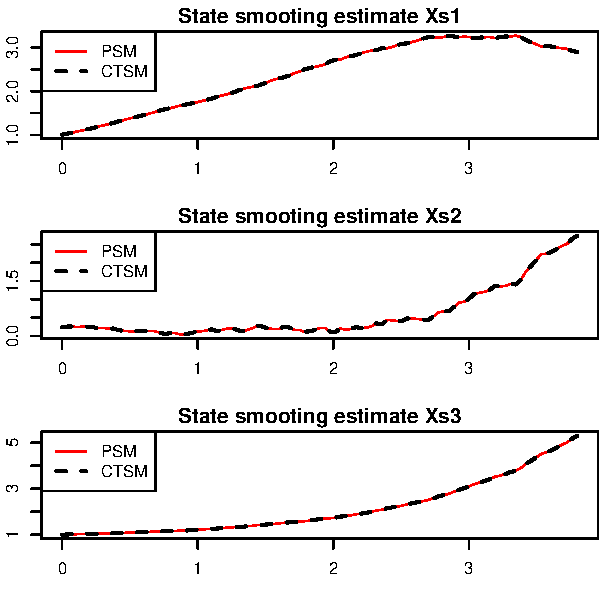
\includegraphics{PSMvsCTSM-figure2}
\end{center}
\caption{Comparison of smoothed estimate of states. }
\label{fig:fig2}
\end{figure}

An exact numerical analysis of the differences can also be performed
as shown in the line below.



\begin{Schunk}
\begin{Sinput}
> (pct <- max(abs(t(CTSMSmooth[, 2:4]) - sm1$Xs)/sm1$Xs * 
+     100))
\end{Sinput}
\begin{Soutput}
[1] 0.07457
\end{Soutput}
\end{Schunk}


 As it can be seen the analysis shows that
smoothed state estimates differ at most 0.075\%.


\small
\begin{thebibliography}{99}
  \addcontentsline{toc}{section}{\refname}
  \bibitem{kristensen03}
    Kristensen NR, Madsen H (2003) Continous time stochastic
    modelling: CTSM 2.3 mathematics guide, Technical University of
    Denmark \\
    http://www2.imm.dtu.dk/ctsm/MathGuide.pdf
  \bibitem{kristensen03b}
    Kristensen NR, Madsen H (2003) Continous time stochastic
    modelling: CTSM 2.3 User's Guide, Technical University of
    Denmark \\
    http://www2.imm.dtu.dk/ctsm/UsersGuide.pdf
  
    
\end{thebibliography}

\end{document}
